\documentclass[10pt,fleqn]{article} % Default font size and left-justified equations
\usepackage[%
    pdftitle={Modélisation systèmes multiphysiques : Modélisation linéaire et non linéaire},
    pdfauthor={Xavier Pessoles}]{hyperref}
    
\input{style/new_style}
\input{style/macros_SII}
\usepackage{multicol}
\usepackage{standalone}
\standaloneconfig{mode=buildnew}
\usepackage{siunitx}
\usepackage{wrapfig}
\fichetrue

%\fichefalse

%\proftrue
%\proffalse

\tdtrue
%\tdfalse

\courstrue
\coursfalse

\def\discipline{Sciences \\Industrielles de \\ l'Ingénieur}
\def\xxtete{Sciences Industrielles de l'Ingénieur}

\def\classe{PSI$\star$}
\def\xxnumpartie{Cy 1 \& 2}
\def\xxpartie{Modéliser le comportement linéaire et non linéaire des systèmes multiphysiques\\
Modéliser les systèmes asservis dans le but de prévoir leur comportement}


\def\xxnumchapitre{}%}Chapitre 1 \vspace{.2cm}}
\def\xxchapitre{}%\hspace{.12cm} Modélisation multiphysique}


\def\xxtitreexo{\noindent }%Micromanipulateur compact pour la chirurgie endoscopique \\ Direction Automobile Découplée}%Motorisation du moteur Haibike}
\def\xxsourceexo{}%\hspace{.2cm} \footnotesize{Mines Ponts 2016 -\item Banque PT SI A 2017 }}


\def\xxposongletx{2}
\def\xxposonglettext{1.45}
\def\xxposonglety{20}
%\def\xxonglet{Part. 1 -\item Ch. 3}
\def\xxonglet{Cy 1 \& 2}

\def\xxactivite{DS 2}
\def\xxauteur{\textsl{Xavier Pessoles}}

\def\xxcompetences{%
\textsl{%
\textbf{Savoirs et compétences :}\\
%Les sources sont associées par un \emph{hacheur série}. La détermination des grandeurs électriques associées à ce montage permet de conclure vis à vis du cahier des charges.
%\noindent \textbf{Résoudre :} à partir des modèles retenus :
%\begin{itemize}[label=\ding{112},font=\color{ocre}] 
%\item choisir une méthode de résolution analytique, graphique, numérique;
%\item mettre en \oe{}uvre une méthode de résolution.
%\end{itemize}
%\begin{itemize}[label=\ding{112},font=\color{ocre}] 
%\item \textit{Rés -\item C1.1 :} Loi entrée sortie géométrique et cinématique -\item Fermeture géométrique.
%\end{itemize}
%
%\noindent \textit{Mod2 -\item C4.1 :} Représentation par schéma-blocs.
}}

\def\xxfigures{
\includegraphics[width=.6\linewidth]{images/fig_01}
}%figues de la page de garde


\def\xxpied{%
Cycle 1 \& 2\\
\xxactivite%
}

\setcounter{secnumdepth}{5}
%---------------------------------------------------------------------------

\usepackage{pgfplots}
\begin{document}
%\defimages{images}
%\chapterimage{png/Fond_Cin}
\input{style/new_pagegarde}
\vspace{7cm}
\pagestyle{fancy}
\thispagestyle{plain}

\def\columnseprulecolor{\color{ocre}}
\setlength{\columnseprule}{0.4pt} 


Un simulateur est un dispositif dont la fonction principale est de reproduire le plus fidèlement possible le comportement d'un système de référence (réel). 
Par rapport à la conduite sur route, les simulateurs de conduite offrent trois avantages majeurs: 
\begin{itemize}
\item ils présentent un environnement sans danger pour le conducteur (par exemple pour tester des accidents virtuels) ; 
\item une même expérience peut être répétée aussi souvent que nécessaire dans des conditions identiques; 
\item ils permettent une économie considérable. 
\end{itemize}
Ainsi, les simulateurs de conduite sont utilisés dans de nombreux domaines : 
\begin{itemize}
\item travaux de recherche sur le comportement humain; 
\item étude et amélioration de la sécurité; 
\item aide à la conception de véhicule ou de l'environnement routier; 
\item apprentissage à moindre coût; 
\item loisir ... 
\end{itemize}
Le simulateur étudié dans ce sujet est un simulateur de course automobile à deux degrés de liberté utilisé par des particuliers dans le domaine du loisir (figure 1). 


\begin{center}
\includegraphics[width=.45\linewidth]{images/fig_01}

\textit{Figure 1 -- Simulateur de course utilisé dans des salles de jeux vidéo.}
\end{center}

Le diagramme SADT de niveau A-0 de la figure 3, %page 3, 
décrit le besoin du simulateur. 
Le diagramme des inter-acteurs de la figure 2, %page 3, 
recense quelques fonctions de service du simulateur. 


\begin{center}
\begin{tabular}{p{.45\linewidth}p{.45\linewidth}}

\begin{center}
\includegraphics[width=.9\linewidth]{images/fig_02}

\end{center}
& 
FS1 : restituer les sensations de conduite au joueur par rapport au sol; 

FS2 : être correctement et solidement positionné sur le sol; 

FS3 : plaire au joueur ; 

FS4 : être d'un encombrement limité par rap¬port à la salle; 

FS5 : être alimenté en énergie. 
\end{tabular}
\textit{Figure 2 -- Diagramme des interacteurs.}
\end{center}
\begin{center}
\includegraphics[width=.9\linewidth]{images/fig_03}

\textit{Figure 3 -- Diagramme SADT de niveau A-0 décrivant le besoin du simulateur de course.}
\end{center}


\begin{center}
\begin{tabular}{p{.45\linewidth}p{.45\linewidth}}
La fonction principale du système peut se décliner en plusieurs fonctions techniques décrites par le diagramme FAST partiel de la figure 4. Les deux premières fonctions sont gérées lors de la conception du jeu vidéo. 
 
& 
\begin{center}
\includegraphics[width=.9\linewidth]{images/fig_04}

\textit{Figure 4 -- Diagramme FAST partiel de la fonction principale du système .}
\end{center}
\end{tabular}



\end{center}

\begin{obj}
Dans ce sujet, seule la fonction technique  << restituer les sensations de mouvement >> sera étudiée pour montrer comment recréer le plus fidèlement possible les accélérations. 
L'objectif de l'étude proposée est de justifier que l'architecture retenue pour le simulateur permet de répondre au besoin. Cette analyse nécessite:
\begin{itemize} 
\item la mise en évidence de la problématique liée à la restitution des accélérations (\ref{sec_1}) ; 
\item la description de l'architecture du système (partie \ref{sec_2}) ; 
\item la mise en place d'un modèle pour chaque constituant de la chaîne d'information (stratégie 
de commande étudiée en partie \ref{sec_3}) et de la chaîne d'énergie (partie \ref{sec_4}) ; 
\item l'utilisation de ces modèles et d'un cahier des charges pour dimensionner les composants (partie \ref{sec_4} et \ref{sec_5}) ; 
\item la détermination du comportement global du système théoriquement et expérimentalement ainsi que la comparaison des performances obtenues par rapport au cahier des charges (partie \ref{sec_5}). 
\end{itemize}
\end{obj}

\section{Mise en évidence de la problématique \label{sec_1}}
La restitution des accélérations est un problème complexe compte-tenu des fonctions contraintes énoncées dans le diagramme des inter-acteurs et de la connaissance imparfaite de la perception humaine. 
Pour mettre en évidence la nécessité d'adopter une stratégie de commande du simulateur particulière, on s'intéresse aux accélérations ressenties lors d'une conduite sur circuit. Le logiciel du jeu vidéo fournit différentes informations dont l'accélération longitudinale (dans le sens d'avance de la voiture) et latérale (voir figure 5) de la voiture par rapport au sol, mais aussi le régime moteur, l'enfoncement des pédales d'accélérateur et de frein. Ces informations sont utiles à deux niveaux: elles servent de consignes d'entrée pour le simulateur mais elles peuvent également être employées pour analyser une course. 


\begin{center}
\includegraphics[width=.9\linewidth]{images/fig_05}

\textit{Figure 5 -- Direction des accélérations longitudinale et latérale.}
\end{center}

La figure 6%,% page 5, 
représente ainsi des données extraites lors d'une course sur une portion de circuit telle que décrite sur la figure 7.%, page 5. 



\subparagraph{}
\textit{Indiquer, en justifiant à l'aide des courbes, pour les zones numérotées 1 à 5 de la figure 6 s'il s'agit d'une zone d'accélération, de freinage, de virage à gauche ou virage à droite. Préciser à quoi correspondent les 2 parties entourées dans la zone 1 (s'aider des autres courbes).}
\ifprof
\begin{corrige}
\end{corrige}
\else
\fi


Les profils typiques d'accélération longitudinale observés pendant la course précédente sont modélisés par des lois trapèzes d'une hauteur d'environ \SI{1}{g} (avec $g = \SI{9,81}{m.s^{-2}}$) pendant $t_m = \SI{3}{s}$ et de temps de montée ou de descente $t_a$ de \SI{0,4}{s} comme indiqué sur la figure 8.%, page 5. 


\subparagraph{}
\textit{Indiquer quelle fonction de service ne sera pas satisfaite compte-tenu des distances calculées. }
\ifprof
\begin{corrige}
\end{corrige}
\else
\fi


\begin{center}
\includegraphics[width=.9\linewidth]{images/fig_06}

\textit{Figure 6 -- Données extraites du jeu vidéo sur une portion de circuit.}
\end{center}


\begin{center}
\begin{tabular}{p{.45\linewidth}p{.45\linewidth}}

\begin{center}
\includegraphics[width=.9\linewidth]{images/fig_07}

\textit{Figure 7 -- Portion de circuit sur lequel sont extraites différentes données.}
\end{center}
& 
\begin{center}
\includegraphics[width=.9\linewidth]{images/fig_08}

\textit{Figure 8 -- Profil d'accélération en trapèze.}
\end{center}

\end{tabular}
\end{center}

Cette étude a permis de montrer qu'il était nécessaire de mettre en place une stratégie de commande de déplacement du siège spécifique qui donne l'illusion au pilote d'être soumis à de telles accélérations. 


\section{Architecture du système \label{sec_2}}
Le SADT de niveau AO du document réponse DR 1 présente l'organisation du simulateur 
étudié. Celui-ci est constitué: 
\begin{itemize}
\item d'une unité centrale munie d'un jeu vidéo et du logiciel de génération de consigne de mouvement; 
\item d'un volant et d'un pédalier; 
\item d'un écran et d'enceintes audio; 
\item d'une structure articulée supportant le siège; 
\item de deux vérins asservis linéaires mettant en mouvement le siège par l'intermédiaire de la structure articulée; 
\item d'un boîtier (nommé SX3000) gérant à la fois l'alimentation des vérins et la communication entre l'unité centrale et les vérins. 
\end{itemize}

\subparagraph{}
\textit{Compléter sur l'ébauche du SADT de niveau A0 du document réponse DR les zones en pointillés en vous aidant de la description du simulateur, du SADT de niveau A-O de la figure 3
%, page 3, 
et de la photo du simulateur de la figure 1.}%, page 2.}
 
\subparagraph{}
\textit{Regrouper les constituants en deux catégories: chaîne d'information et chaîne d'énergie. Un élément, de par sa constitution, sera placé dans les deux chaînes.} 

\section{Stratégie de commande\label{sec_3}}

La structure articulée possède deux degrés de liberté (roulis et tangage) comme indiqué sur la figure 9. La partie I a montré qu'il est indispensable de mettre au point une stratégie de commande des degrés de liberté qui permette de recréer les accélérations subies par le pilote pour respecter un encombrement réduit. 

\begin{center}
\includegraphics[width=.9\linewidth]{images/fig_09}

\textit{Figure 9 -- Mouvements de tangage et roulis permettant de générer des accélérations longitudinale et transversale.}
\end{center}

La stratégie de commande classique est basée sur une séparation fréquentielle des accélérations extraites du jeu vidéo en deux parties. 
Le schéma-bloc de la figure 10%, page 7, 
montre le principe de la commande sur l'angle de tangage $\alpha$. 

\textbf{Dans tout le sujet, seules les accélérations longitudinales (commande de l'angle de tangage) seront considérées. Une stratégie similaire est adoptée pour l'angle de roulis.}

\begin{center}
\includegraphics[width=.9\linewidth]{images/fig_10}

\textit{Figure 10 -- Stratégie de commande pour un mouvement de tangage.}
\end{center}

\begin{obj}
L'objectif de cette partie est de déterminer les fonctions de transfert intervenant dans ce schéma-blocs et de vérifier que cette méthode permet de fournir une consigne d'angle adaptée à l'encombrement du simulateur. La vérification globale de la stratégie vis-à-vis de la restitution des accélérations longitudinales sera faite en fin de sujet. 
\end{obj}

\subsection{Principe}
On note $\rep{0}\repere{O}{x_0}{y_0}{z_0}$ le repère associé au sol \textbf{(0)}, supposé galiléen. Le paramétrage est défini sur la figure 11. L'ensemble \{conducteur + siège\} est noté \textbf{(1)} et est en rotation par rapport au sol \textbf{(0)} autour d'un axe $\axe{O}{y_0}$. 
On associe le repère $\rep{1}\repere{O}{x_1}{y_1}{z_1}$ à l'ensemble 
\textbf{(1)} et on note $\alpha =\angl{x_0}{x_1} =\angl{z_0}{z_1} $) l'angle de tangage de \textbf{(1)} par rapport à \textbf{(0)}. 


\begin{center}
\includegraphics[width=.9\linewidth]{images/fig_11}

\textit{Figure 11 -- Paramétrage pour le mouvement de tangage seul et figure de calcul.}
\end{center}


Un point de la tête proche de l'oreille interne du pilote noté $A$ est défini par: $\vect{OA} = h\vect{z_1}$. L'accélération de la pesanteur est $\vect{g} = -g\vect{z_0}$ avec $g = \SI{9,81}{m.s^{-2}}$. 

Le siège est piloté de telle manière que l'accélération donnée par le jeu vidéo soit équivalente à l'accélération ressentie par le pilote sur le siège. En notant $\vect{a_T}$ l'accélération du véhicule, on obtient la définition suivante: 
$\vect{a_T}=a_{Tx} \vect{x_1}+a_{Tz} \vect{z_1}=\vectg{A}{1}{0}-\vect{g}$.



\subparagraph{}
\textit{Montrer que : $$ \begin{array}{l}a_{Tx}=h\ddot{\alpha} - g \sin \alpha \\a_{Tz}=-h\dot{\alpha}^2 - g \cos\alpha \end{array}.$$}

\ifprof
\begin{corrige}
\end{corrige}
\else
\fi


Dans la stratégie adoptée, l'accélération ressentie $a_{Tx}$ est décomposée en deux parties $a_{Tx} = a_{\text{mov}} + a_{\text{tilt}}$. La composante $a_{\text{tilt}}$ correspond à la partie de l'accélération maintenue tandis que la composante $a_{\text{mov}}$ caractérise les variations rapides d'accélération. 

\subsection{Obtention de l'accélération $a_{\text{tilt}}$}

La partie $a_{\text{tilt}}$ est extraite de $a_{Tx}$ en utilisant un filtre $H_{\text{tilt}}$ caractérisé par les diagrammes de Bode de la figure 12. Elle représente les mouvements maintenus dans le temps. 


\begin{center}
\includegraphics[width=.9\linewidth]{images/fig_12}

\textit{Figure 12 -- Diagrammes de Bode du filtre modélisé par la fonction de transfert $H_{\text{tilt}}(p)$.}
\end{center}

\subparagraph{}\textit{Proposer une forme de fonction de transfert pour la fonction $H_{\text{tilt}}(p)$ en fonction de ces diagrammes de Bode et identifier ses paramètres caractéristiques. }

Pour reproduire ce type de mouvement, compte-tenu des limitations structurelles du simulateur, on incline le siège d'un angle $\alpha_{\text{tilt}}$ de manière à orienter le pilote par rapport au vecteur pesanteur de façon à ce qu'il ressente une accélération $a_{Tx}$. Si ce mouvement est couplé avec un défilement des images adéquat, le pilote a la sensation d'être dans un véhicule d'accélération $a_{Tx}$.

\subparagraph{}\textit{En utilisant l'expression de $a_{Tx}$ obtenue précédemment à la Q6, déterminer, en régime établi (dérivées nulles), l'expression de l'angle de coordination $\alpha_{\text{tilt}}$, en fonction de g et $a_{Tx}$ . }

Si l'angle de coordination $\alpha_{\text{tilt}}$ n'est pas trop important, le pilote ne ressent pas la diminution d'accélération verticale (composante $a_{Tz}$) et n'a pas l'impression de tomber. En effet, le système vestibulaire de l'oreille interne du pilote est sensible à des variations d'accélérations supérieures à environ $\pm \SI{0,25}{m.s^{-2}}$ selon la direction verticale. 

\subparagraph{}\textit{Donner les valeurs extrêmes (en degré) que peut prendre $\alpha_{\text{tilt}}$ afin que la variation d'accélération verticale $ \left|a_{Tz} - g\right|$ (variation par rapport à l'accélération verticale de référence $g$) ne dépasse pas la valeur seuil de détection de l'oreille interne en régime établi.}

\subparagraph{}\textit{En déduire la valeur maximale d'accélération longitudinale $a_{Tx}$ qu'il est possible de simuler avec cette méthode en régime établi. Déterminer alors le gain d'adaptation $K_{\text{adapt}}> 0$ du schéma-blocs à prendre, sachant que les accélérations extrêmes $a_{Tx\text{, jeu}}$ délivrées par le logiciel de jeu sont de $\pm \SI{10}{m.s^{-2}}$.}


\subsection{Détermination de l'accélération $a_{\text{mov}}$}

Le filtre utilisé pour accéder à la partie $a_{\text{mov}}$ a pour fonction de transfert $H_{\text{mov}} (p)= \dfrac{\tau p}{1+\tau p}$. On choisit une valeur de $\tau = \SI{0,1}{s}$. 


\subparagraph{}\textit{Tracer sur le document réponse DR 2 les diagrammes de Bode asymptotiques et l'allure des diagrammes réels de ce filtre. Préciser le nom de ce filtre et son intérêt vis-à-vis de la composante à extraire. }

Une fois l'accélération filtrée, on obtient la relation $a_{\text{mov}}=h\ddot{a}_{\text{mov}}$.

\subparagraph{}\textit{En déduire la fonction de transfert $H_{\text{mov2}}(p)$.}

En imposant une consigne $a_{Tx} = a_0 u(t)$ où $a_0$ est une constante et $u(t)$ la fonction échelon unitaire, on obtient les courbes $a_{\text{mov}}$ et $\alpha_{\text{mov}}$ définies sur la figure 13. 


\begin{center}
\includegraphics[width=.9\linewidth]{images/fig_13}

\textit{Figure 13 -- Accélération $a_{\text{mov}}$ et $\alpha_{\text{mov}}$  en fonction du temps (en s) pour une consigne d'accélération en échelon.}
\end{center}


\subparagraph{}\textit{À partir de la fonction de transfert $H_{\text{mov2}}(p)$ et de la consigne en échelon imposée, justifier l'allure des courbes obtenues par simulation en régime établi et conclure sur la nécessité de choisir un filtre plus élaboré.}


On modifie donc la fonction $H_{\text{mov2}}$ en la multipliant par un filtre particulier appelé filtre Washout ayant pour but de ramener à zéro la position linéaire obtenue pour une accélération $a_{Tx}$ constante. 

En choisissant un filtre adapté, on retient la fonction globale suivante: $H_{\text{mov1}}(p)\times H_{\text{mov2}}(p)=\dfrac{K_p}{\left(\tau p+1\right)^3}$.


\subparagraph{}\textit{Montrer alors qu’en régime permanent, l’angle $\alpha_{\text{mov}}$ obtenu pour une accélération $a_{Tx}$ de type échelon (de valeur $\alpha_0$) est nul.}

La stratégie de commande complète est testée pour une accélération longitudinale trapèze définie sur la figure 8. 
On obtient les résultats de simulation de la figure 14 permettant, entre autre, d'observer l'allure de l'angle de tangage à appliquer ainsi que les accélérations $a_{Tx}$ et $a_{Tz}$ obtenues pour cet angle de tangage. 



\begin{center}
\includegraphics[width=.9\linewidth]{images/fig_14}

\textit{Figure 14 -- Résultats de simulation pour une accélération longitudinale en trapèze.}
\end{center}

\subparagraph{}\textit{Justifier le signe de l'angle $\alpha$. Commenter les niveaux constants des accélérations $a_{Tx}$ et $a_{Tz}$ vis-à-vis de la réponse attendue à partir des différentes valeurs calculées dans cette partie.}

La loi de commande proposée permet de définir une consigne d'angle à suivre pour restituer l'accélération donnée par le jeu. Cependant, des stratégies plus élaborées sont en réalité employées pour obtenir des courbes d'accélérations plus « régulières ». 

\section{Dimensionnement et modélisation du simulateur \label{sec_4}}
La partie précédente a permis de définir la loi de mouvement souhaitée pour le siège. Le cahier des charges, associé à la fonction technique FT3 «restituer les sensations de mouvement», qui se décline en la fonction technique « générer un mouvement angulaire donné», est précisé dans le tableau 1. 

\begin{obj}
L'objectif de cette partie est de mettre en place une modélisation de la chaîne d'énergie du simulateur de manière à vérifier le respect de la loi angulaire déterminée précédemment. La mise en place de ce modèle permettra également de dimensionner les constituants pour respecter le cahier des charges. 
\end{obj}


\begin{center}
\begin{tabular}{|l|l|}
\hline
Critères & Niveaux \\ \hline
Débattement angulaire & $\pm 13\degres$ \\ \hline
Accélération extrême $a_{Tx}$ (définie dans la suite)& $\pm \SI{2,2}{m.s^{-2}}$ \\ \hline
 Masse du conducteur admissible & \SI{100}{kg} \\ \hline
Rapidité & $t_{5\%} < \SI{0,1}{s}$ pour une entrée en échelon \\ \hline
Précision& Erreur nulle en réponse à une consigne en échelon \\ 
& Erreur constante en réponse à une consigne en rampe \\ \hline
Stabilité & Absolue \\ \hline
Dépassement 	& $< 20\%$ \\ \hline
\end{tabular}

\textit{Tableau 1: Extrait du cahier des charges.}
\end{center}

\subsection{Modélisation de la structure articulée}
La cinématique retenue pour le simulateur est basée sur une structure articulée permettant deux degrés de liberté par l'intermédiaire de deux vérins linéaires asservis. On désigne par \textbf{(3a)} et \textbf{(3b)} les corps des vérins en liaison sphérique avec le châssis noté \textbf{(0)}, \textbf{(2a)} et \textbf{(2b)} les tiges des vérins en liaison sphérique avec le siège noté \textbf{(1)}, lui même en liaison avec le châssis. Les tiges des vérins sont en liaison glissière avec les corps des vérins. La liaison entre le siège et le châssis est réalisée par un joint de cardan \textbf{(C)} qui autorise deux rotations (selon les axes $\axe{O}{x_0}$ et $\axe{O}{y_0}$). 

Le graphe des liaisons (figure 15) synthétise les modèles de liaisons utilisés pour cette structure. Ce graphe fait référence aux points et axes définis sur l'épure du schéma cinématique donné dans le document réponse DR3.




\begin{center}
\includegraphics[width=.9\linewidth]{images/fig_15}

\textit{Figure 15 -- Graphe des liaisons de la structure articulée .}
\end{center}

\subparagraph{}
\textit{À l'aide du graphe des liaisons, compléter le schéma cinématique en perspective du document réponse DR3 en respectant les axes et points proposés.}

\subparagraph{}
\textit{Lorsque les vérins sont à mi-course, l'assise du siège est horizontale. Renseigner dans le tableau du document réponse DR 4, par un signe + (une tige de vérin sort) ou un signe - (une tige de vérin rentre), le comportement des vérins a et b pour obtenir un mouvement de tangage dans le sens direct ou un mouvement de roulis dans le sens direct. Le vérin a est le vérin situé à l'arrière gauche du conducteur. }

\subparagraph{}
\textit{Déterminer le degré d'hyperstatisme du modèle ainsi proposé en précisant bien les mobilités utiles et internes. Indiquer l'intérêt d'une telle modélisation vis-à-vis de la détermination des efforts dans le système. Préciser un autre intérêt de ce degré d'hyperstatisme.}


Dans toute la suite de l'étude, on ne s'intéressera qu'au mouvement de tangage (rotation autour de $\vect{y_0}$). Dans ces conditions, il est possible de trouver un modèle plan équivalent du mécanisme. Le vérin est alors appelé vérin équivalent. 

La figure 16 correspond à cette modélisation plane équivalente. Le paramétrage est donné sur cette figure. $\alpha$ est l'angle de tangage du siège par rapport au châssis. Dans toute la suite du problème, on ne s'intéressera qu'à ce modèle plan. 


\begin{center}
\includegraphics[width=.9\linewidth]{images/fig_16}

\textit{Figure 16 -- Modèle plan du simulateur pour l'étude du mouvement de tangage.}
\end{center}

Le modèle établi va permettre de vérifier le dimensionnement des vérins vis-à-vis des critères du cahier des charges. 


\subsection{Critère de débattement angulaire}

La partie III a montré que, pour restituer correctement les accélérations, il fallait que le débattement angulaire du siège soit limité. Pour respecter le critère de débattement angulaire, la course des vérins doit être adaptée. 

\subparagraph{}
\textit{Par une fermeture géométrique, exprimer $\lambda$ en fonction de $\alpha$ ainsi que des dimensions constantes du système puis exprimer $\beta$ en fonction de $\alpha$ et des mêmes dimensions.}
 
On donne dans le document réponse DR 5 les courbes obtenues à partir des deux relations déterminées précédemment. Lorsque l'assise du siège est horizontale, l'angle $\alpha$ est nul, le vérin est alors à mi course (la longueur $\lambda$ est de \SI{0,99}{m}). La course du vérin équivalent est de \SI{0,15}{m}, $\lambda$ peut donc varier de $\pm \SI{0,075}{m}$ autour de $\SI{0,99}{m}$. 

\subparagraph{}
\textit{Déterminer le débattement angulaire et comparer la valeur obtenue à celle du cahier des charges.}





On approche les deux courbes par des droites au voisinage de $\alpha=0\degres$ : $\lambda = \lambda_0 + K_{\alpha}$ et $\beta = \beta_0 + K_{\beta} \alpha$. 

\subparagraph{}
\textit{En utilisant les courbes du document réponse DR 5, donner les valeurs numériques de $K_{\alpha}$, $K_{\beta}$ et $\beta_0$. Conserver les unités définies sur les figures.}

Le modèle ainsi établi permettra de relier dans la suite la commande des vérins à l'angle souhaité du siège. 

\subsection{Critère de masse admissible}
D'après les données du constructeur, le vérin équivalent peut développer un effort maximal de 
$\pm \SI{200}{N}$ environ. On cherche dans cette partie à vérifier si le vérin est capable de mettre en mouvement le siège sur lequel serait assis un conducteur ayant la masse définie dans le cahier des charges. 
On définit les grandeurs cinétiques et géométriques suivantes : 
\begin{itemize}
\item $J = \SI{10}{kg. m^2}$, moment d'inertie de l'ensemble \{conducteur + siège\} selon l'axe $\left(O,\vect{y_0}\right)$; 
\item $m = \SI{100}{kg}$, masse de l'ensemble \{conducteur + siège\} ; 
- 
\item $\vect{OG} = d\vect{z_1}$ avec $d = \SI{0,35}{m}$ : position du centre de gravité de l'ensemble \{conducteur + siège\} (position simplifiée pour limiter les calculs). 
\end{itemize}
On note: 
\begin{itemize}
\item $-g \vect{z_0}$ avec $9 = \SI{9,81}{m.s^{-2}}$, accélération de la pesanteur; 
\item $F\vect{x_3}$ l'action mécanique de la tige du vérin équivalente \textbf{(2)} sur le siège \textbf{(1)} se modélise par un glisseur en $A$. 
\end{itemize}

\subparagraph{}
\textit{En isolant le vérin équivalent \{tige \textbf{(2)} + corps \textbf{(2)}\} de la figure 16, %page 12, 
justifier que l'effort exercé par ce vérin équivalent est dirigé selon $\vect{x_3}$. La masse du vérin et ses caractéristiques inertielles seront supposées négligeables.}


\subparagraph{}
\textit{Déterminer une équation reliant les quantités définies ci-dessus et l'angle a ainsi que ses dérivées sous la forme:  $A_s\dfrac{\dd^2 \alpha(t)}{\dd t^2}=B_S \times F \cos \left(\beta - \alpha\right)+C_s \sin \alpha$ 
où l'on donnera l'expression de $A_s$, $B_s$ et $C_s$ en fonction des paramètres constants. 
Pour cela, préciser le système isolé. Faire le bilan des actions mécaniques et indiquer l'équation du principe fondamental de la dynamique utilisée (résultante / moment, direction, point). }

Le cahier des charges définit un angle maximal de $\pm 13\degres$. 
L'accélération $a_{Tx}$ ressentie par le conducteur indiquée dans ce cahier des charges de $\pm \SI{2,2}{m.s^{-2}}$ est égale à $a_{Tx} = h\ddot{\alpha} - g\sin(\alpha)$ d'après la question Q6. 
On prend les valeurs numériques suivantes: $A_s = \SI{10}{kg.m^2}$, $B_s = \SI{0,7}{m}$ et $C_s = \SI{350}{Nm}$. 

\subparagraph{}
\textit{En déduire l'expression de la force du vérin $F$ en fonction de $a_{Tx}$, $\alpha$, $\beta$, $g$, $A_s$, $B_s$ et $C_s$. Effectuer l'application numérique dans les conditions les plus défavorables ($\alpha = 13\degres$, accélération $a_{Tx}= - \SI{2,2}{m.s^{-2}}$), la valeur de $\beta$ sera lue sur la courbe du document réponse DR 5. Conclure quant au choix de ce vérin.}



\subsection{Modèle de l'ensemble en mouvement}

Le vérin électrique est constitué d'un moteur électrique dont le rotor est lié à la vis d'un dispositif vis-écrou de pas $P_v = \SI{3}{mm.tour^{-1}}$. L'écrou est solidaire de la tige du vérin. Le moteur exerce un couple $C_{\text{mot}}$ sur la vis. On note $\omega_{\text{mot}}$ la vitesse angulaire de la vis solidaire du rotor du moteur noté (mot) ($\theta_{\text{mot}}$) est l'angle de rotation de la vis). 

\subparagraph{}
\textit{Donner le coefficient $k_T$ tel que $\dot{\alpha}=\omega_{\text{mot}} k_T$ en fonction de $P_v$ et $K_{\alpha}$ (défini en Q21). }

On suppose dans la suite que: $\alpha = k_T\theta_{\text{mot}}$. 
On isole tout le simulateur {siège + conducteur et vérin}. On garde le modèle cinématique plan de la figure 16, %page 12, 
composé d'un unique vérin. 
Le moment d'inertie de l'ensemble \{rotor + vis du vérin\} autour de son axe est noté $J_{\text{mot}}= 4 \times 10^{-6}\text{kg\,m}^2$. Le moment d'inertie de l'ensemble \{siège + conducteur\} est noté $J = \SI{10}{kg.m^2}$. Les autres quantités inertielles sont négligées. 
On suppose de plus que $\dot{\beta} = 0$.
 
Les frottements visqueux sont modélisés par un couple $C_v(t) = -f_v \omega_{\text{mot}(t)}$ appliqué sur le rotor du moteur (mot) du vérin équivalent. On suppose que les liaisons sont parfaites. L'action de la pesanteur n'est prise en compte que sur l'ensemble \{siège + conducteur\} de masse $m$. 

\subparagraph{}
\textit{Déterminer l'expression de l'énergie cinétique $E_c$; du simulateur dans le référentiel galiléen \textbf{(0)} et en déduire l'inertie équivalente $J_e$ de ce système ramenée sur l'arbre moteur, telle que $E_c=\dfrac{1}{2}J_e \omega_{mot}^2$. Faire l'application numérique.}

\subparagraph{}
\textit{Déterminer l'expression des puissances extérieures et intérieures qui s'appliquent sur le simulateur. }

\subparagraph{}
\textit{Montrer que la relation obtenue par l'application du théorème de l'énergie cinétique après linéarisation (angle a petit) et simplification est: $J_e \dot{\omega}_{\text{mot}} =C_{\text{mot}}-f_v {\omega}_{\text{mot}} + K{\theta}_{\text{mot}}$ où l'on précisera l'expression de $K$ en fonction de $k_T$, $m$, $d$ et $g$.}
 
Le moteur est commandé en courant de telle sorte que ${C}_{\text{mot}}(t) = k_i i(t)$, où $i(t)$ est l'intensité dans le moteur. 

\subparagraph{}
\textit{Déterminer la fonction de transfert de la chaîne d'énergie en supposant les conditions de Heaviside: $H_{\text{mot}}(p)=\dfrac{{\theta}_{\text{mot}}(p)}{I(p)}$ où $I(p)$ et ${\theta}_{\text{mot}}(p)$ sont les transformées de Laplace de $i(t)$ et ${\theta}_{\text{mot}}(t)$.}

La mise en place d'un modèle plan pour le mouvement de tangage a permis d'une part de vérifier que le vérin était bien dimensionné pour respecter le cahier des charges et d'autre part de déterminer une fonction de transfert reliant la commande des moteurs au déplacement angulaire du siège. 


\section{Mise en place de l'asservissement \label{sec_5}}
\begin{obj}
L'objectif de cette dernière partie est de mettre en place l'asservissement du vérin et de justifier le choix du correcteur pour respecter les consignes d'angles. \end{obj}

On se réfèrera aux éléments du cahier des charges définis en début de partie \ref{sec_4}.
 
L'angle de rotation du moteur est mesuré par un capteur de gain $K_c$. L'image de l'angle de rotation donnée par le capteur est comparée à une grandeur image de l'angle de tangage de consigne $\alpha_c$ fournie par un adaptateur de gain $K_a$. L'écart $\varepsilon(t)$ correspondant est corrigé par un correcteur + amplificateur de fonction de transfert $C(p)$ pour fournir l'intensité de commande 
$i(t)$ au moteur. On rappelle que $H_{\text{mot}}(P) = \dfrac{\theta_{\text{mot}}(p)}{I(p)}$ et que $\alpha(p) = k_T \theta_{\text{mot}}(p)$. 

\subparagraph{}
\textit{Proposer un schéma-blocs de la structure d'asservissement d'entrée $\alpha_c(p)$ et de sortie $\alpha(p)$.} 

\subparagraph{}
\textit{Déterminer l'expression du gain $K_a$ permettant d'obtenir une erreur $\alpha_c-\alpha$ proportionnelle à l'écart $\varepsilon(t)$. Montrer que le schéma-blocs d'asservissement peut alors être ramené à un schéma-blocs à retour unitaire de la forme de la figure 17, avec $H(p)$ à préciser.}

\begin{center}
\includegraphics[width=.9\linewidth]{images/fig_17}

\textit{Figure 17 -- Schéma-blocs à retour unitaire équivalent au schéma-bloc du système.}
\end{center}


Dans toute la suite du sujet, on utilisera la fonction, en unités S.I.,
$ 
H(p) = \dfrac{1}{1,4 \times 10^{-5}p^2 + 10^{-3}p - 0,00035}$. 
On retient un correcteur de la forme $C(p)=\dfrac{\left(1+Tp\right)^2}{Tp}$.
En choisissant judicieusement les paramètres $T$ et $K_{\text{cor}}$ du correcteur, on assure la stabilité 
du système en boucle fermée. 

\subparagraph{}
\textit{Justifier que le système est précis en réponse à une entrée échelon et que l'erreur est finie en réponse à une entrée en rampe de pente unitaire. Donner l'expression de cette erreur.}

On donne dans le document réponse DR 6 les réponses théoriques à un échelon de \SI{0,1}{rad} et à une rampe de pente \SI{0,1}{rad.s^{-1}} pour un réglage satisfaisant du correcteur. 

\subparagraph{}
\textit{Vérifier que le système est stable, que la précision est cohérente avec la question précédente (donner les valeurs des erreurs) et déterminer le temps de réponse à 5\, \% ainsi que la valeur du premier dépassement. Les tracés devront être faits sur le document réponse DR 6. Conclure quant à la satisfaction du cahier des charges.}



\section{Synthèse}
\subparagraph{}
\textit{En vous servant du schéma-bloc de la figure 10% page 7, 
rappeler en deux ou trois phrases le principe de commande des vérins ou d'obtention d'une loi de tangage donnée.}

Un essai est réalisé sur le système en situation pour une consigne d'accélération en trapèze. 
On mesure à l'aide d'un accéléromètre l'accélération en un point du siège mis en mouvement par les vérins. On obtient la courbe de la figure 18 avec les accélérations en $\text{ms}^{-2}$. 


\begin{center}
\includegraphics[width=.9\linewidth]{images/fig_18}

\textit{Figure 18 -- Comparaison des réponses simulées et expérimentales en fonction du temps (s).}
\end{center}

\subparagraph{}
\textit{Commenter l'allure des accélérations simulée et mesurée par rapport à l'accélération de consigne. Indiquer une source de différences compte-tenu des explications données à la question précédente.}

La figure 19 rappelle la démarche de l'ingénieur qui consiste à caractériser les écarts entre 3 domaines (celui du cahier des charges (jeu), de l'expérience et de la modélisation). 

\begin{center}
\includegraphics[width=.9\linewidth]{images/fig_19}

\textit{Figure 19 -- Démarche de l'ingénieur.}
\end{center}


\subparagraph{}
\textit{Indiquer à quelle(s) question(s) de la partie IV, les écarts 1 à 3 ont été caractérisés. Préciser les critères de performances définis dans le cahier des charges relatif à la fonction FT3 qui ont été analysés dans ces questions.}


 
\newpage 


\begin{center}
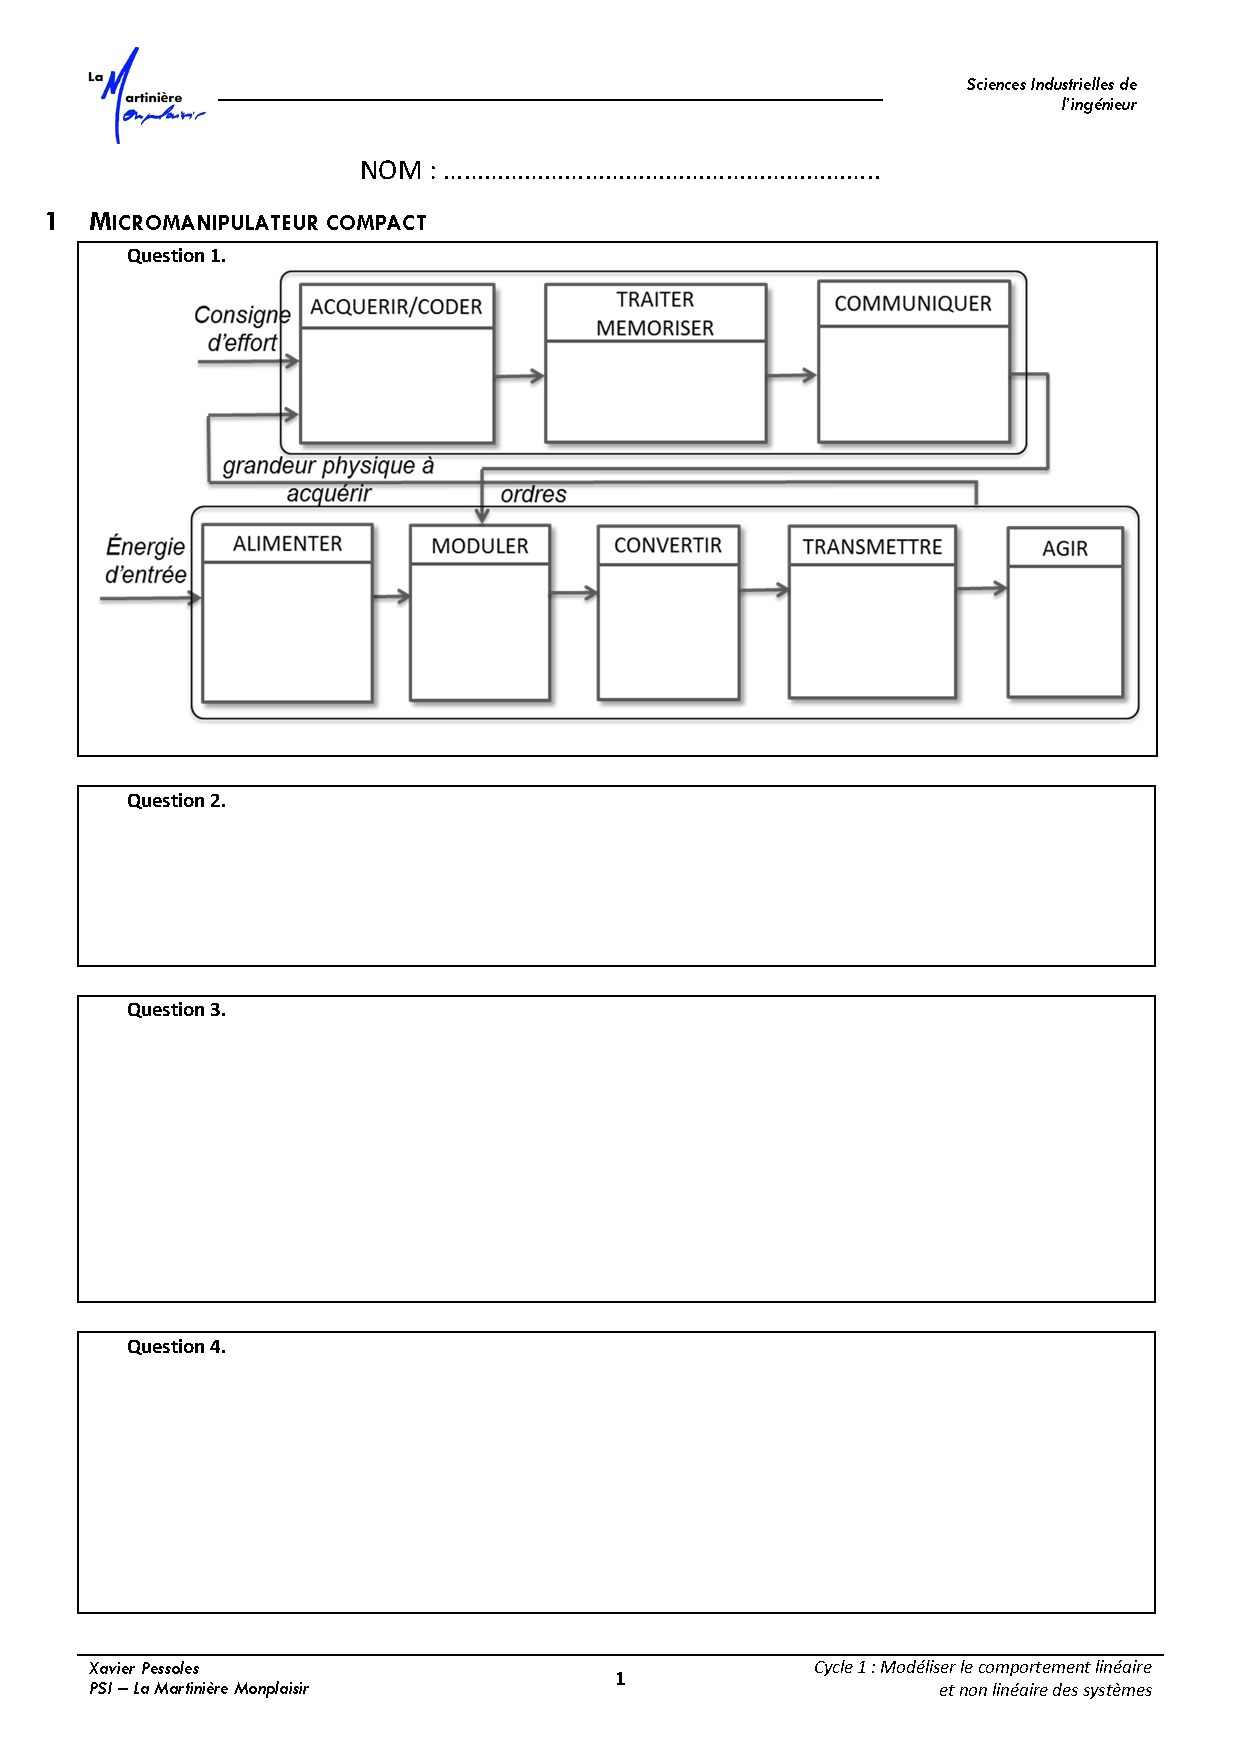
\includegraphics[width=.9\linewidth]{images/DR_01}

\textit{DR 1 -- SADT de niveau A0 du simulateur de course.}
\end{center}

\begin{center}
\includegraphics[width=.9\linewidth]{images/DR_02}

\textit{DR 2 -- Diagramme de Bode du filtre de la fonction de transfert $H_{\text{mov1}}(p)=\dfrac{\tau p}{1+\tau p}$.}
\end{center}

\begin{center}
\includegraphics[width=.9\linewidth]{images/DR_03}

\textit{DR 3 -- Schéma cinématique de la structure articulée.}
\end{center}

\begin{center}
\includegraphics[width=.9\linewidth]{images/DR_04}

\textit{DR 4 -- Tableau du mouvement du siège en fonction du déplacement des vérins.}
\end{center}

\begin{center}
\includegraphics[width=.9\linewidth]{images/DR_05}

\textit{DR 5 -- Longueur du vérin et angle $\beta$ en fonction de l'angle $\alpha$.}
\end{center}

\begin{center}
\includegraphics[width=.9\linewidth]{images/DR_06}

\includegraphics[width=.9\linewidth]{images/DR_06_b}

\textit{DR 6 -- Réponses simulées pour des entrées en échelon et en rampe.}
\end{center}

\end{document}

\subparagraph{}
\textit{}
\ifprof
\begin{corrige}
\end{corrige}
\else
\fi
  